\section{Future Work}

This lays the foundation for future work, where we will focus on formalizing a
collection of general data management policies that can be used across domains
and services. The value of such a collection eases the burden of policy
development and paves the way for solutions that remove the administrator from
the development cycle, such as (1) adaptable policies that automatically switch
to new strategies when the current strategy behaves poorly ({e.g.}, thrashing,
making no progress, etc.), and (2) policy generation, where new policies are
constructed automatically by examining the collection of existing policies.
Such work is made possible with Mantle's ability to dynamically change
policies.

\section{Conclusion}
\begin{figure}[tb]
  \noindent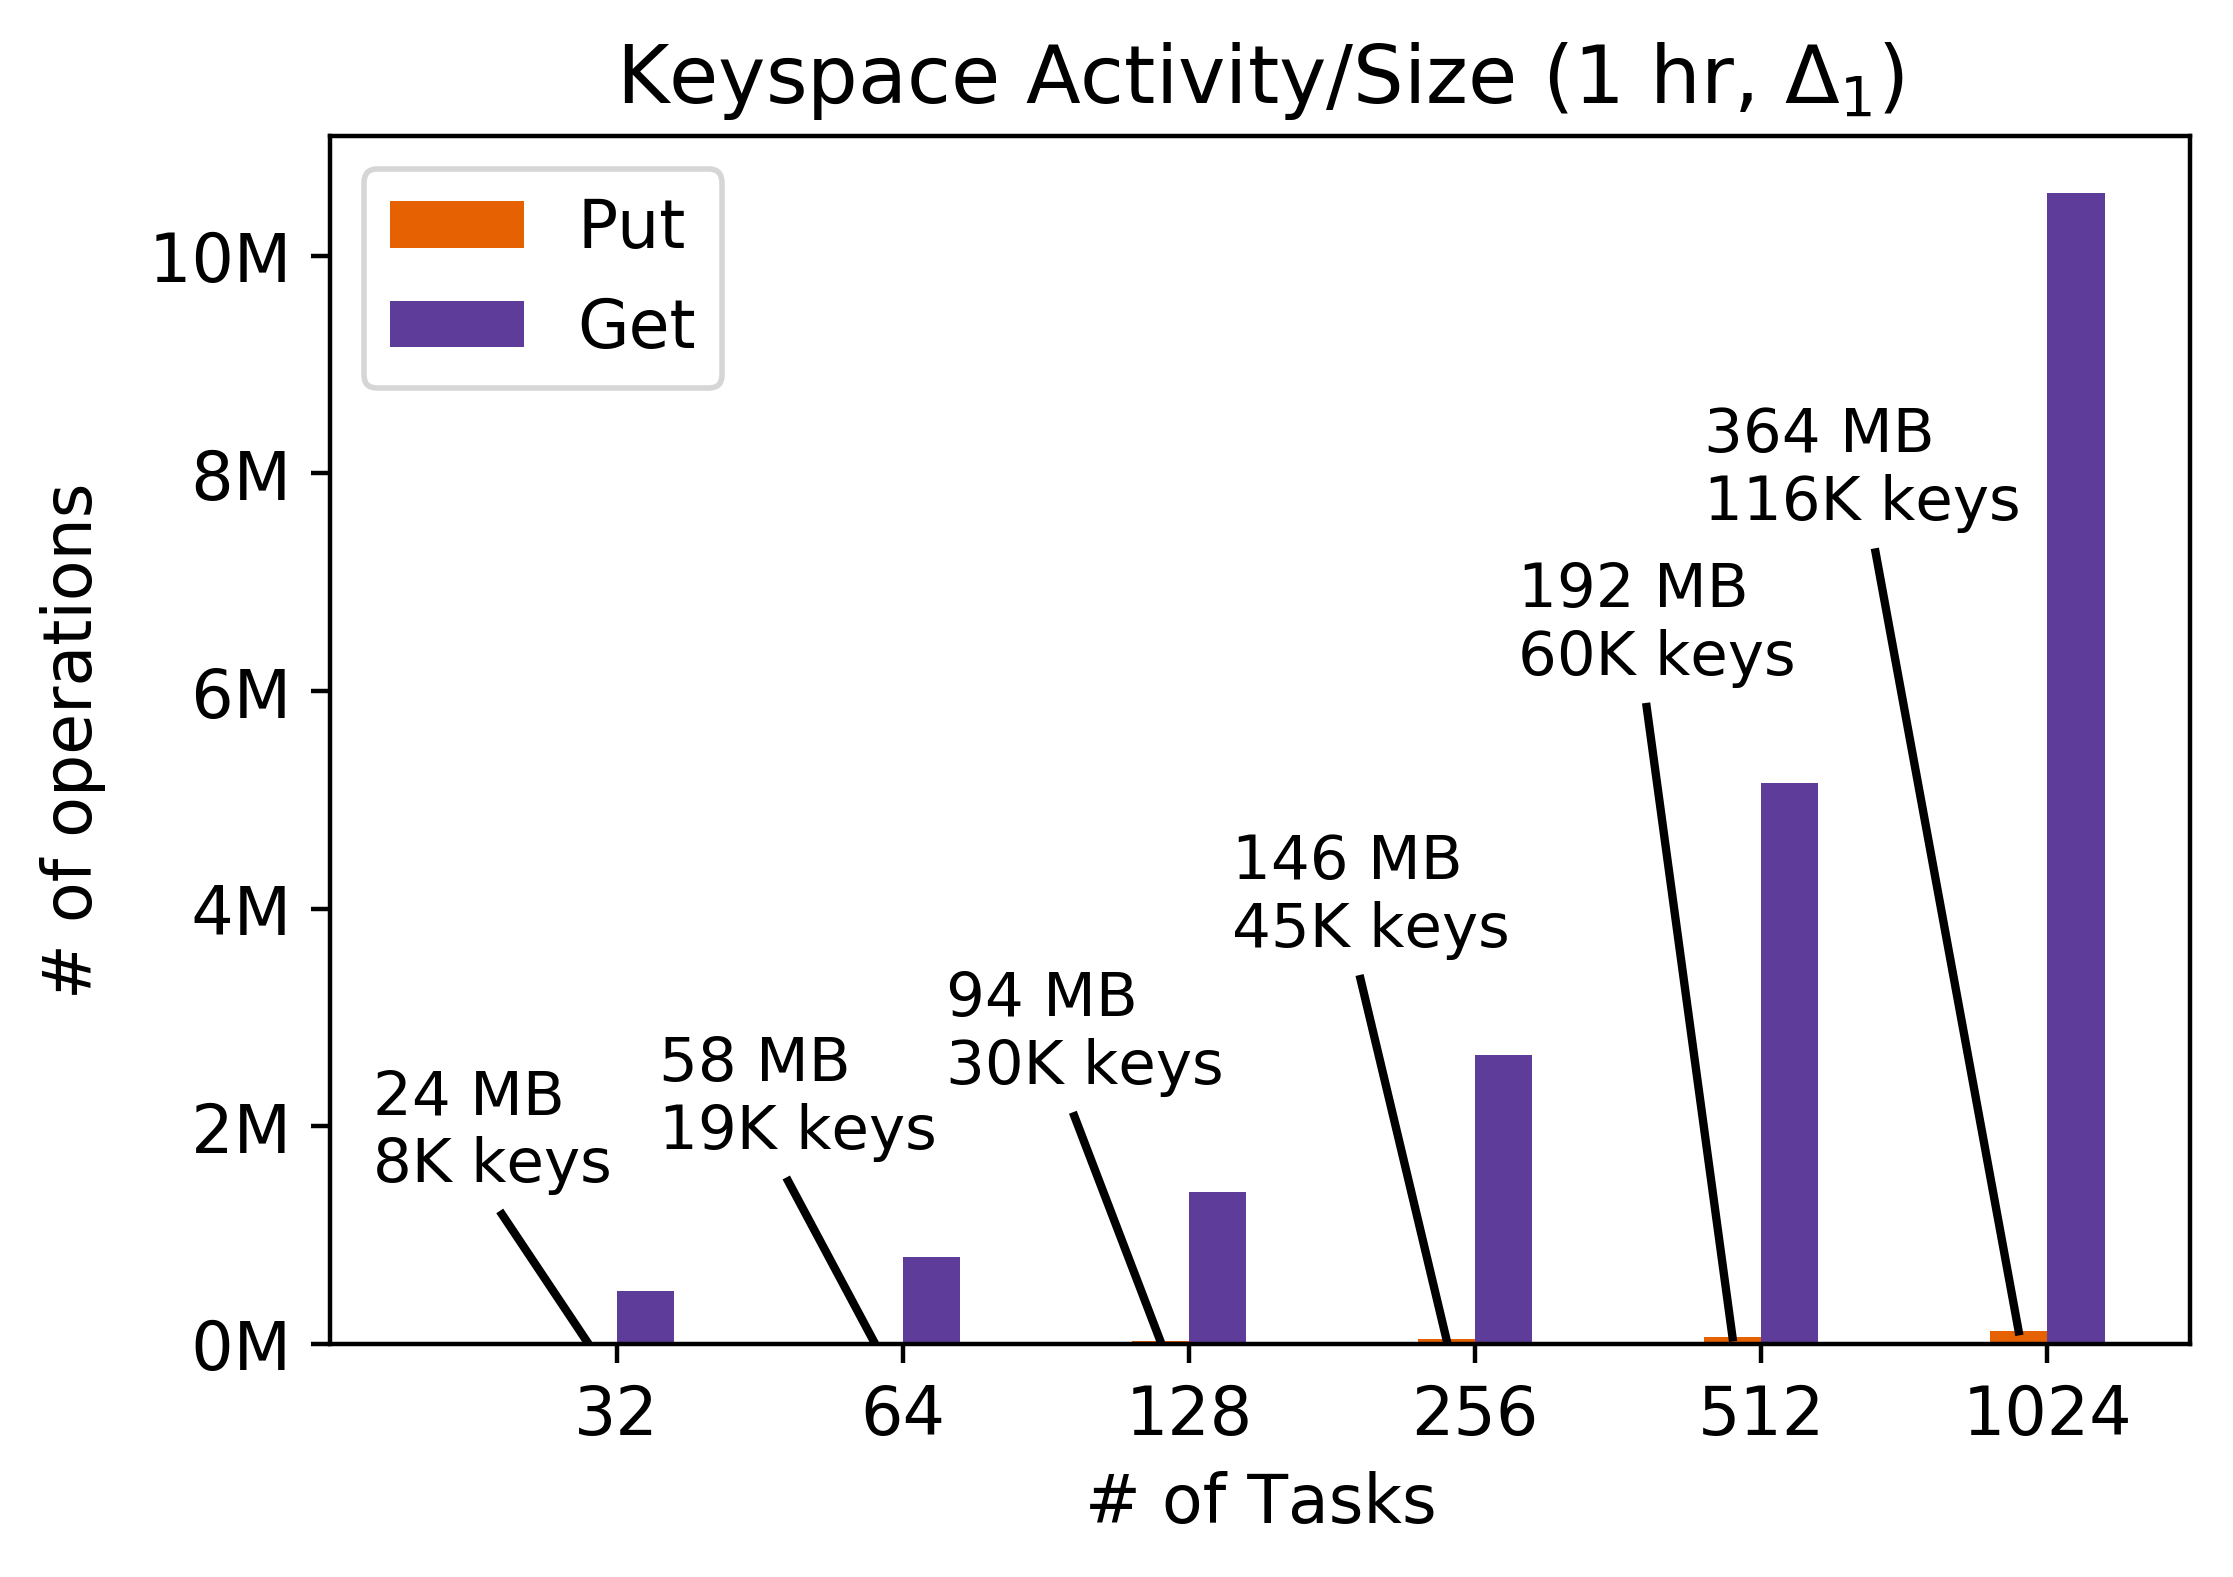
\includegraphics[width=0.5\textwidth]{figures/keyspace-analysis_size.png}\\
  \caption{\label{fig:keyspace-analysis_size}}
\end{figure}
\begin{figure}[tb]
  \noindent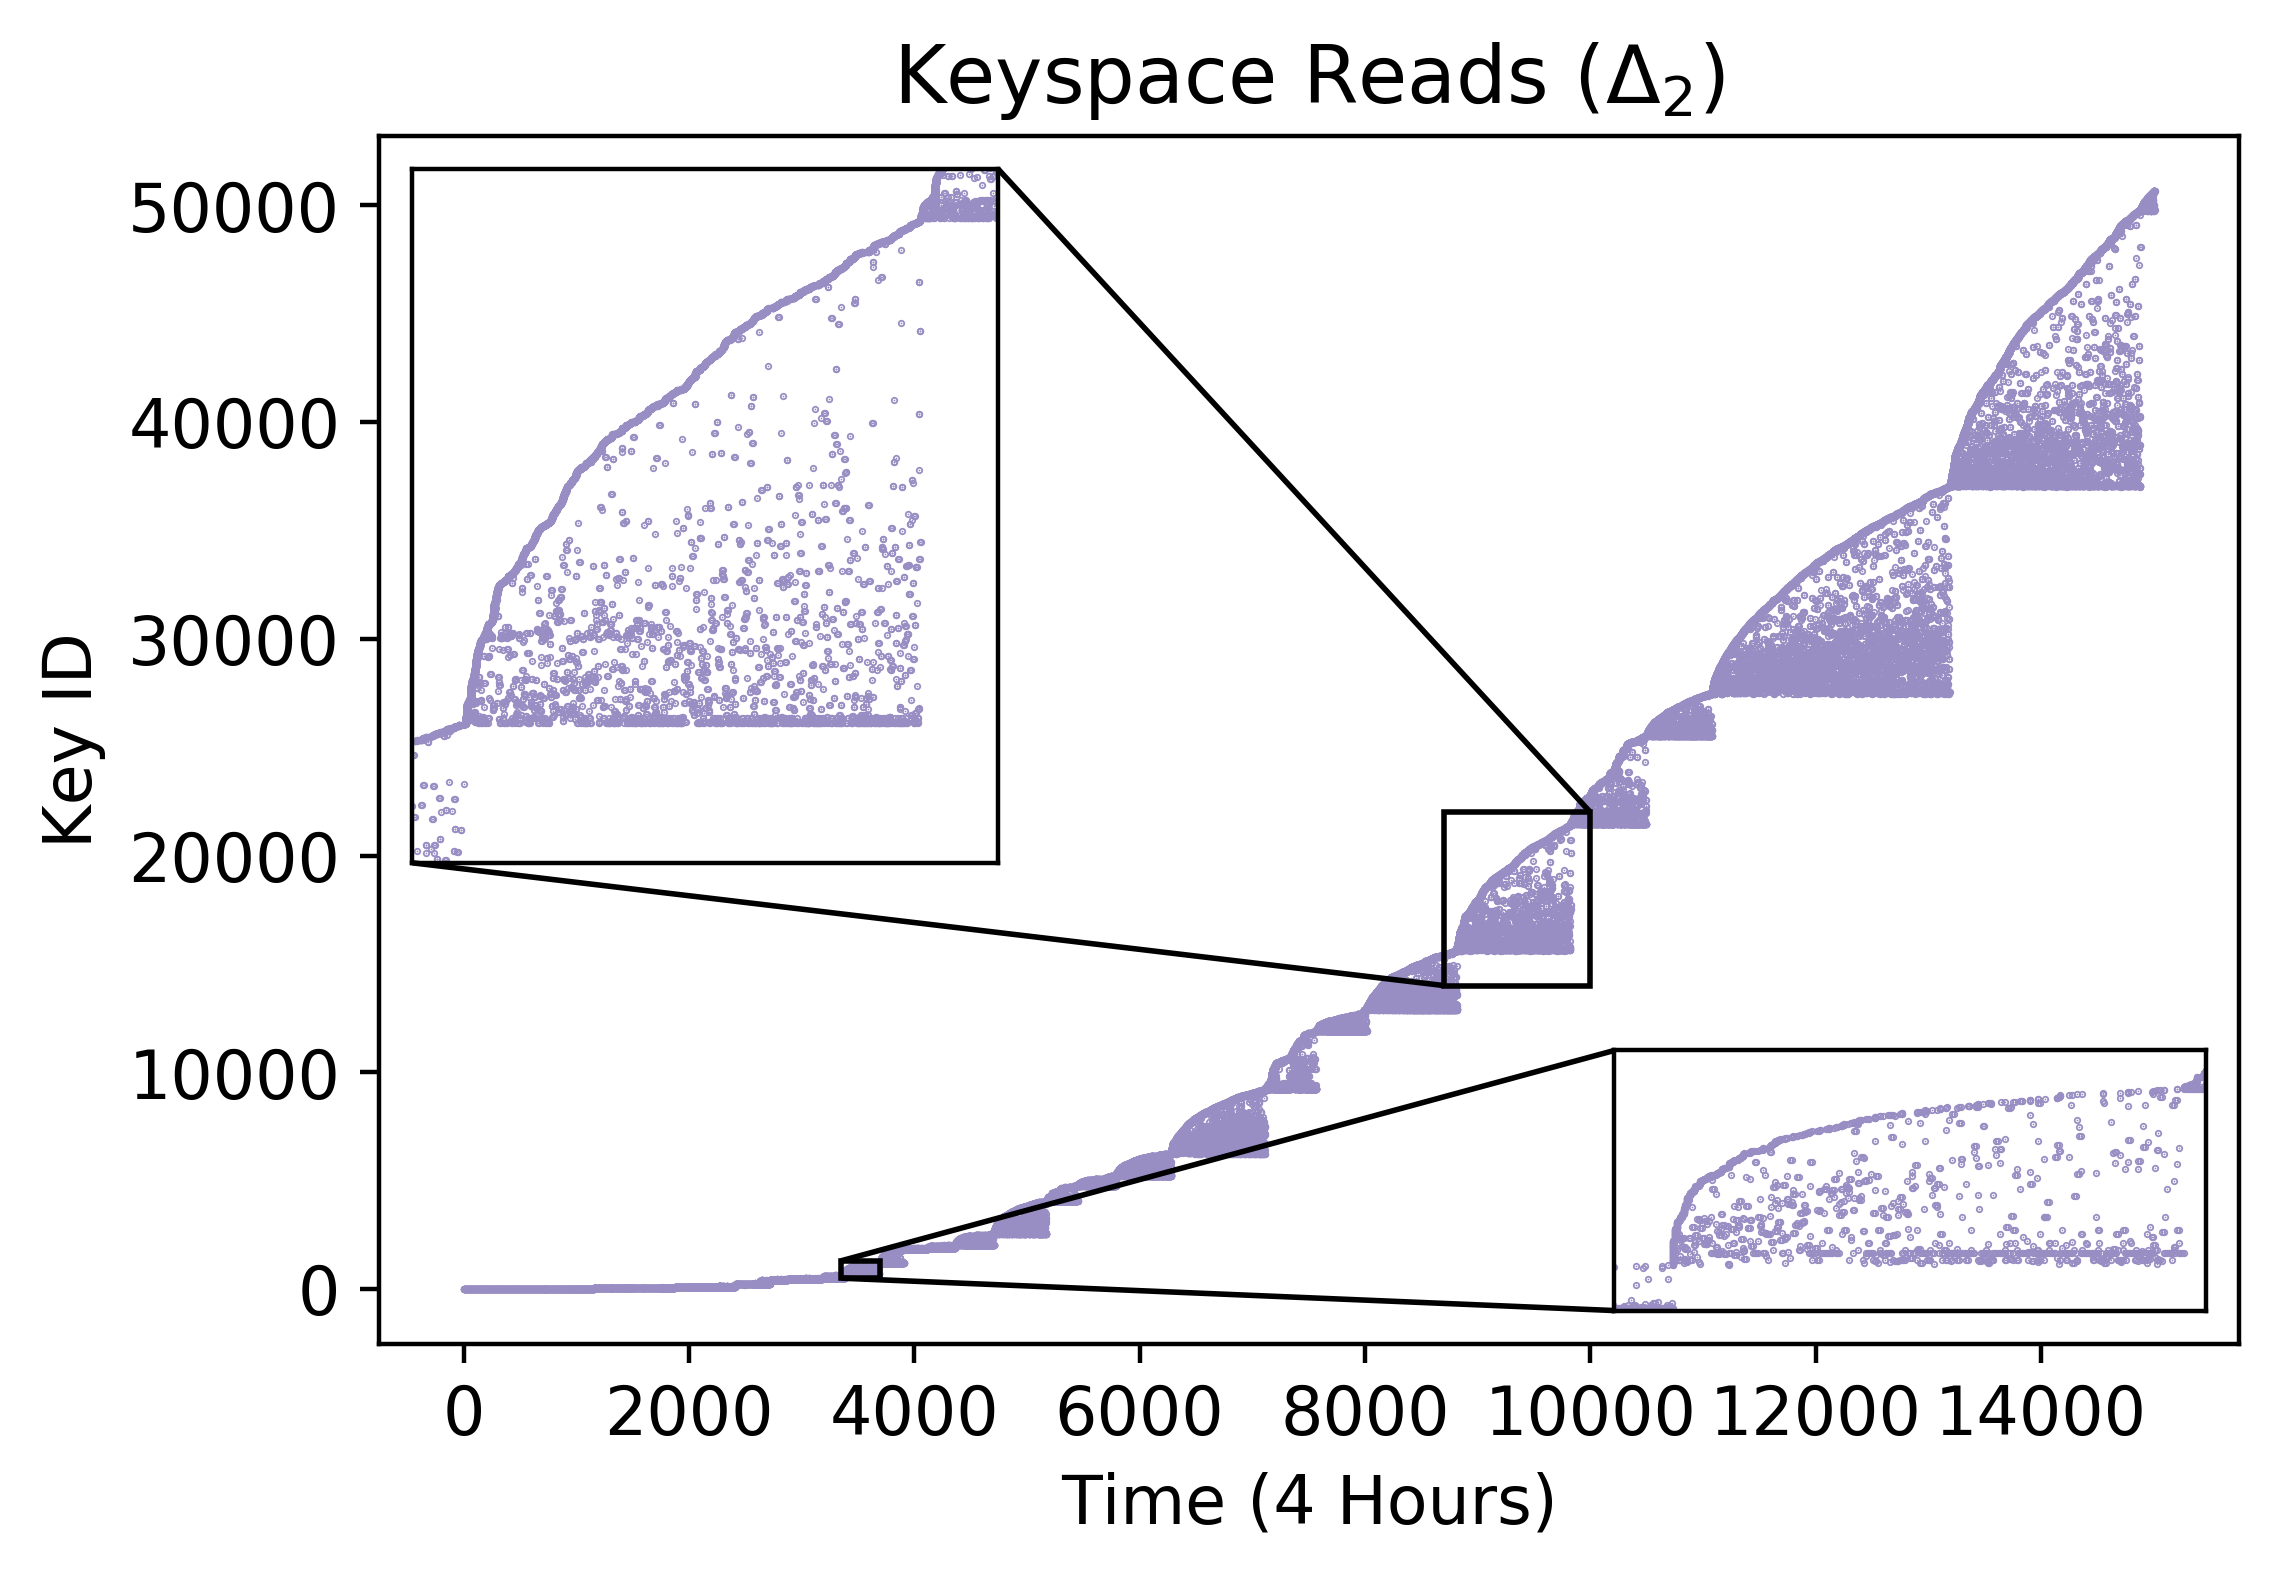
\includegraphics[width=0.5\textwidth]{figures/keyspace-analysis_locality.png}\\
  \caption{\label{fig:keyspace-analysis_locality}}
\end{figure}
\begin{figure}[tb]
  \noindent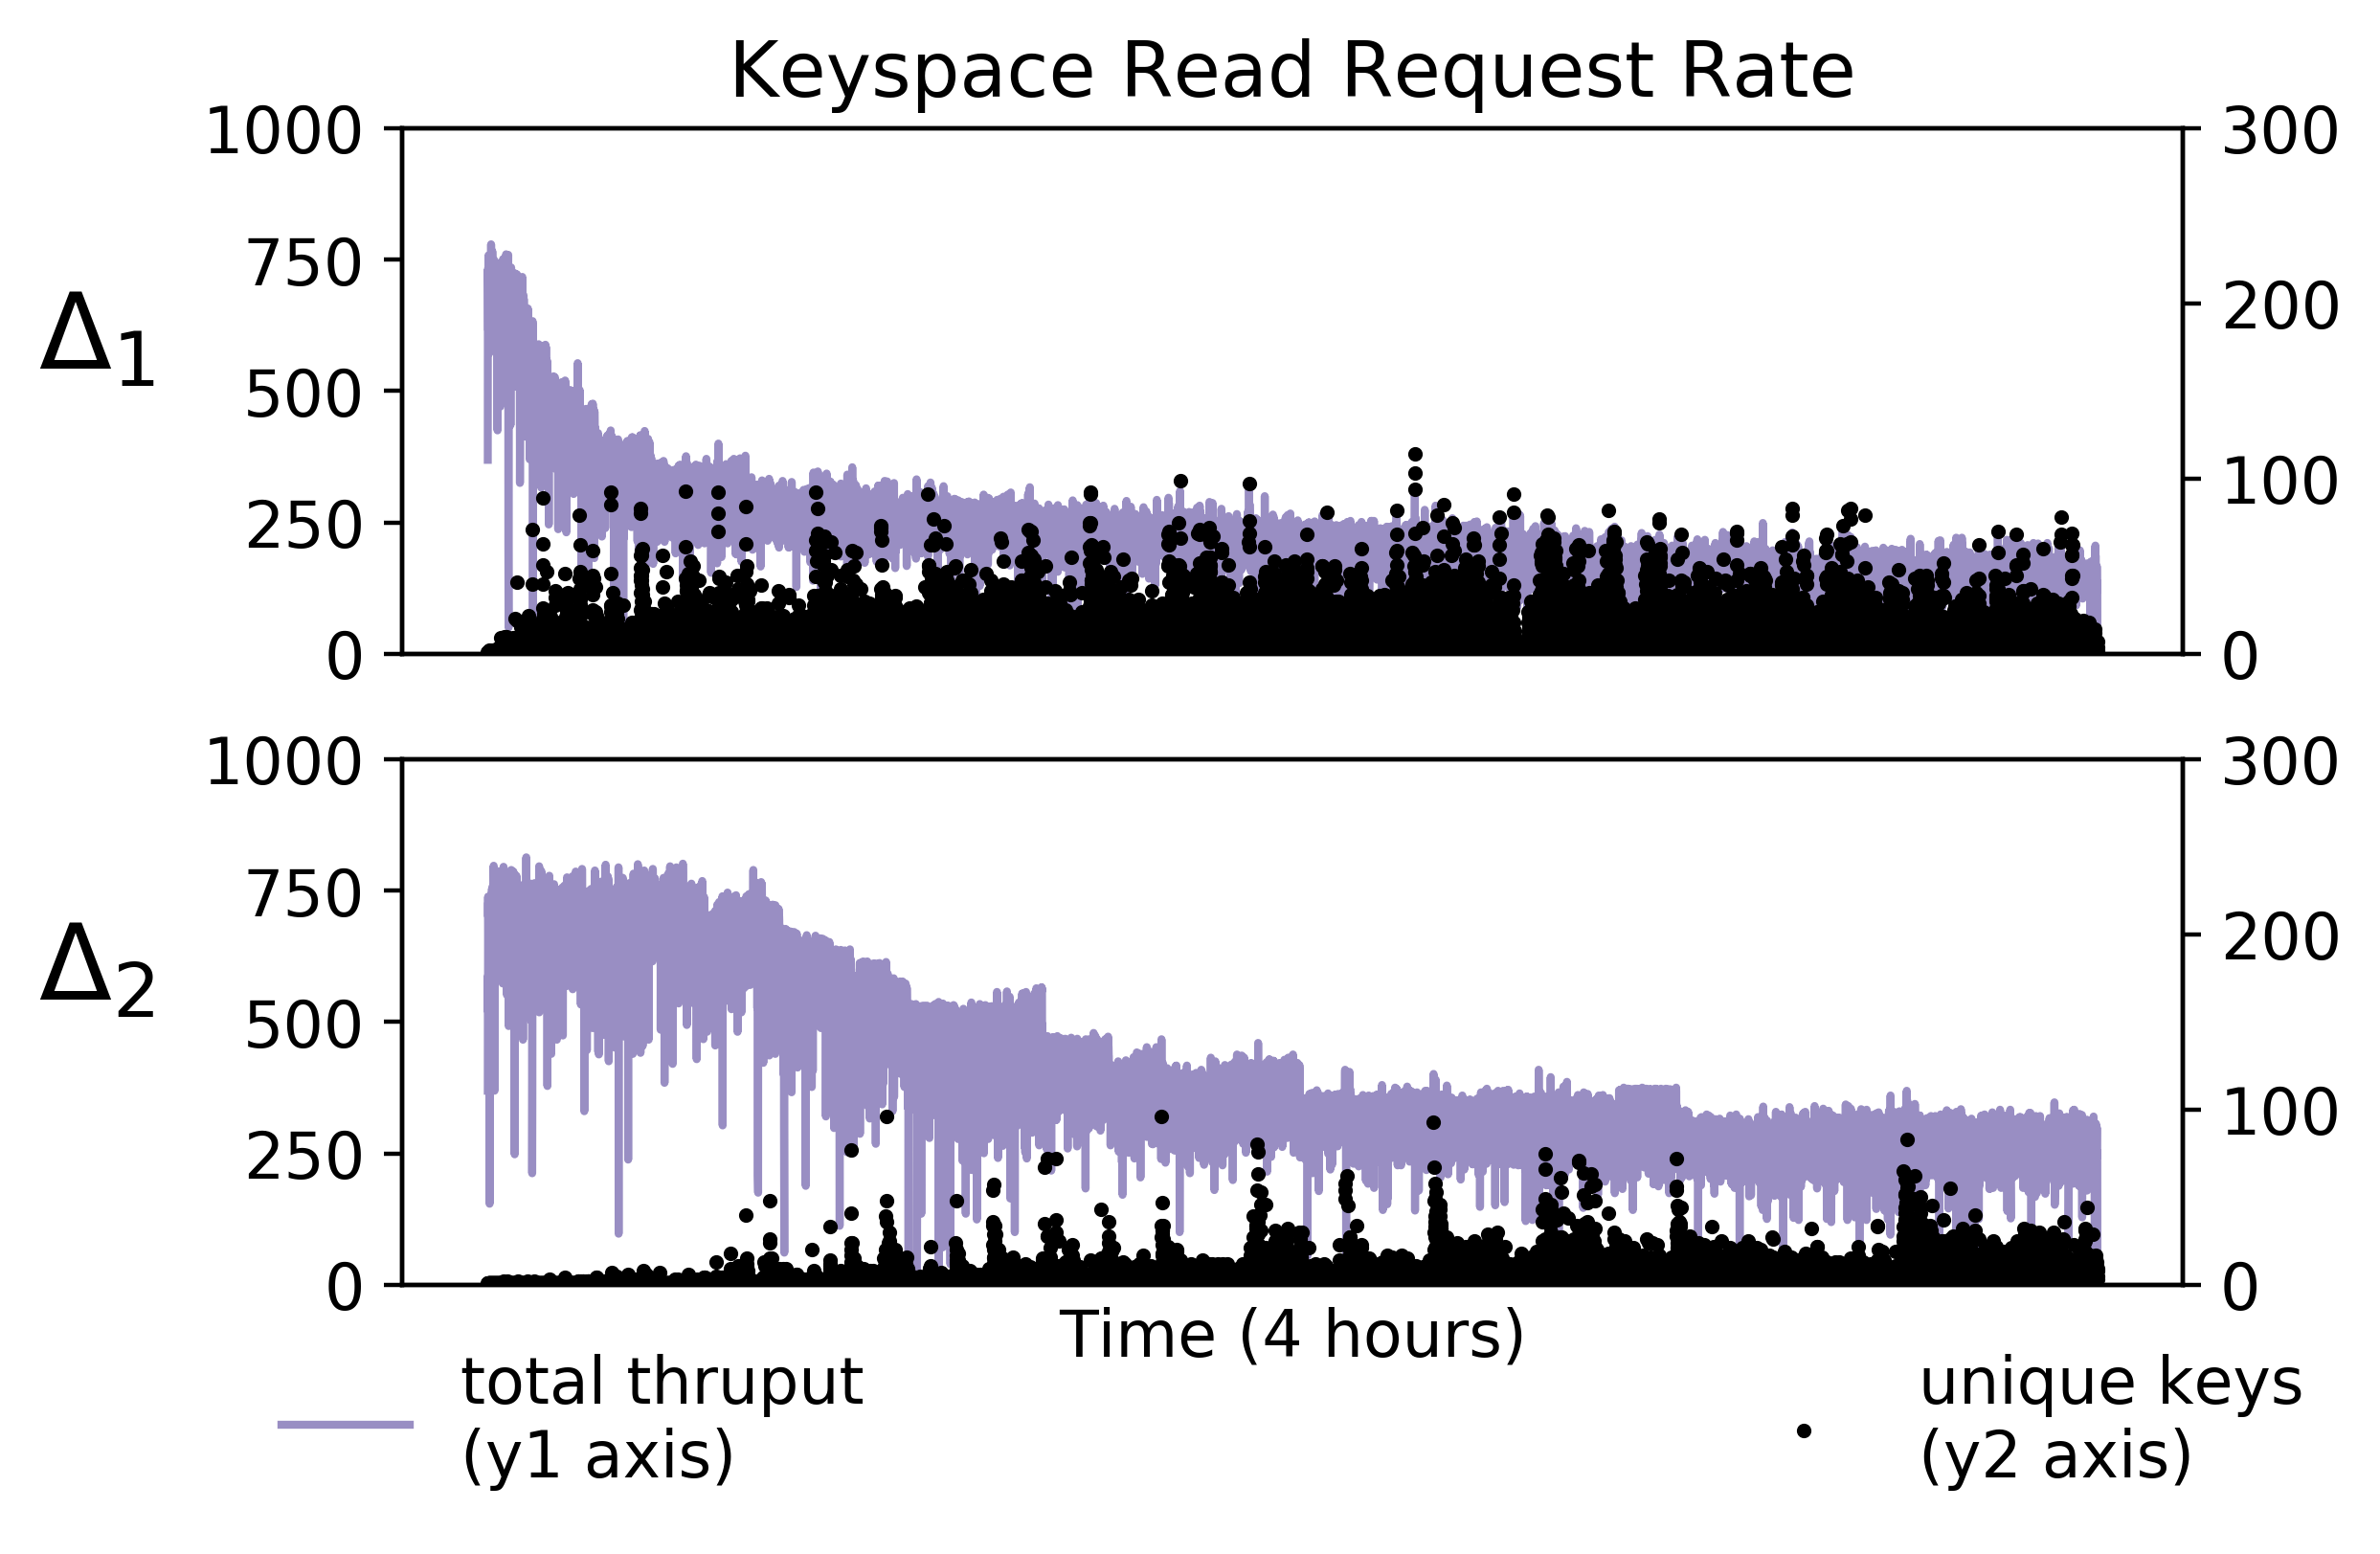
\includegraphics[width=0.5\textwidth]{figures/keyspace-analysis_throughput.png}\\
  \caption{\label{fig:keyspace-analysis_throughput}}
\end{figure}
\begin{figure}[tb]
  \noindent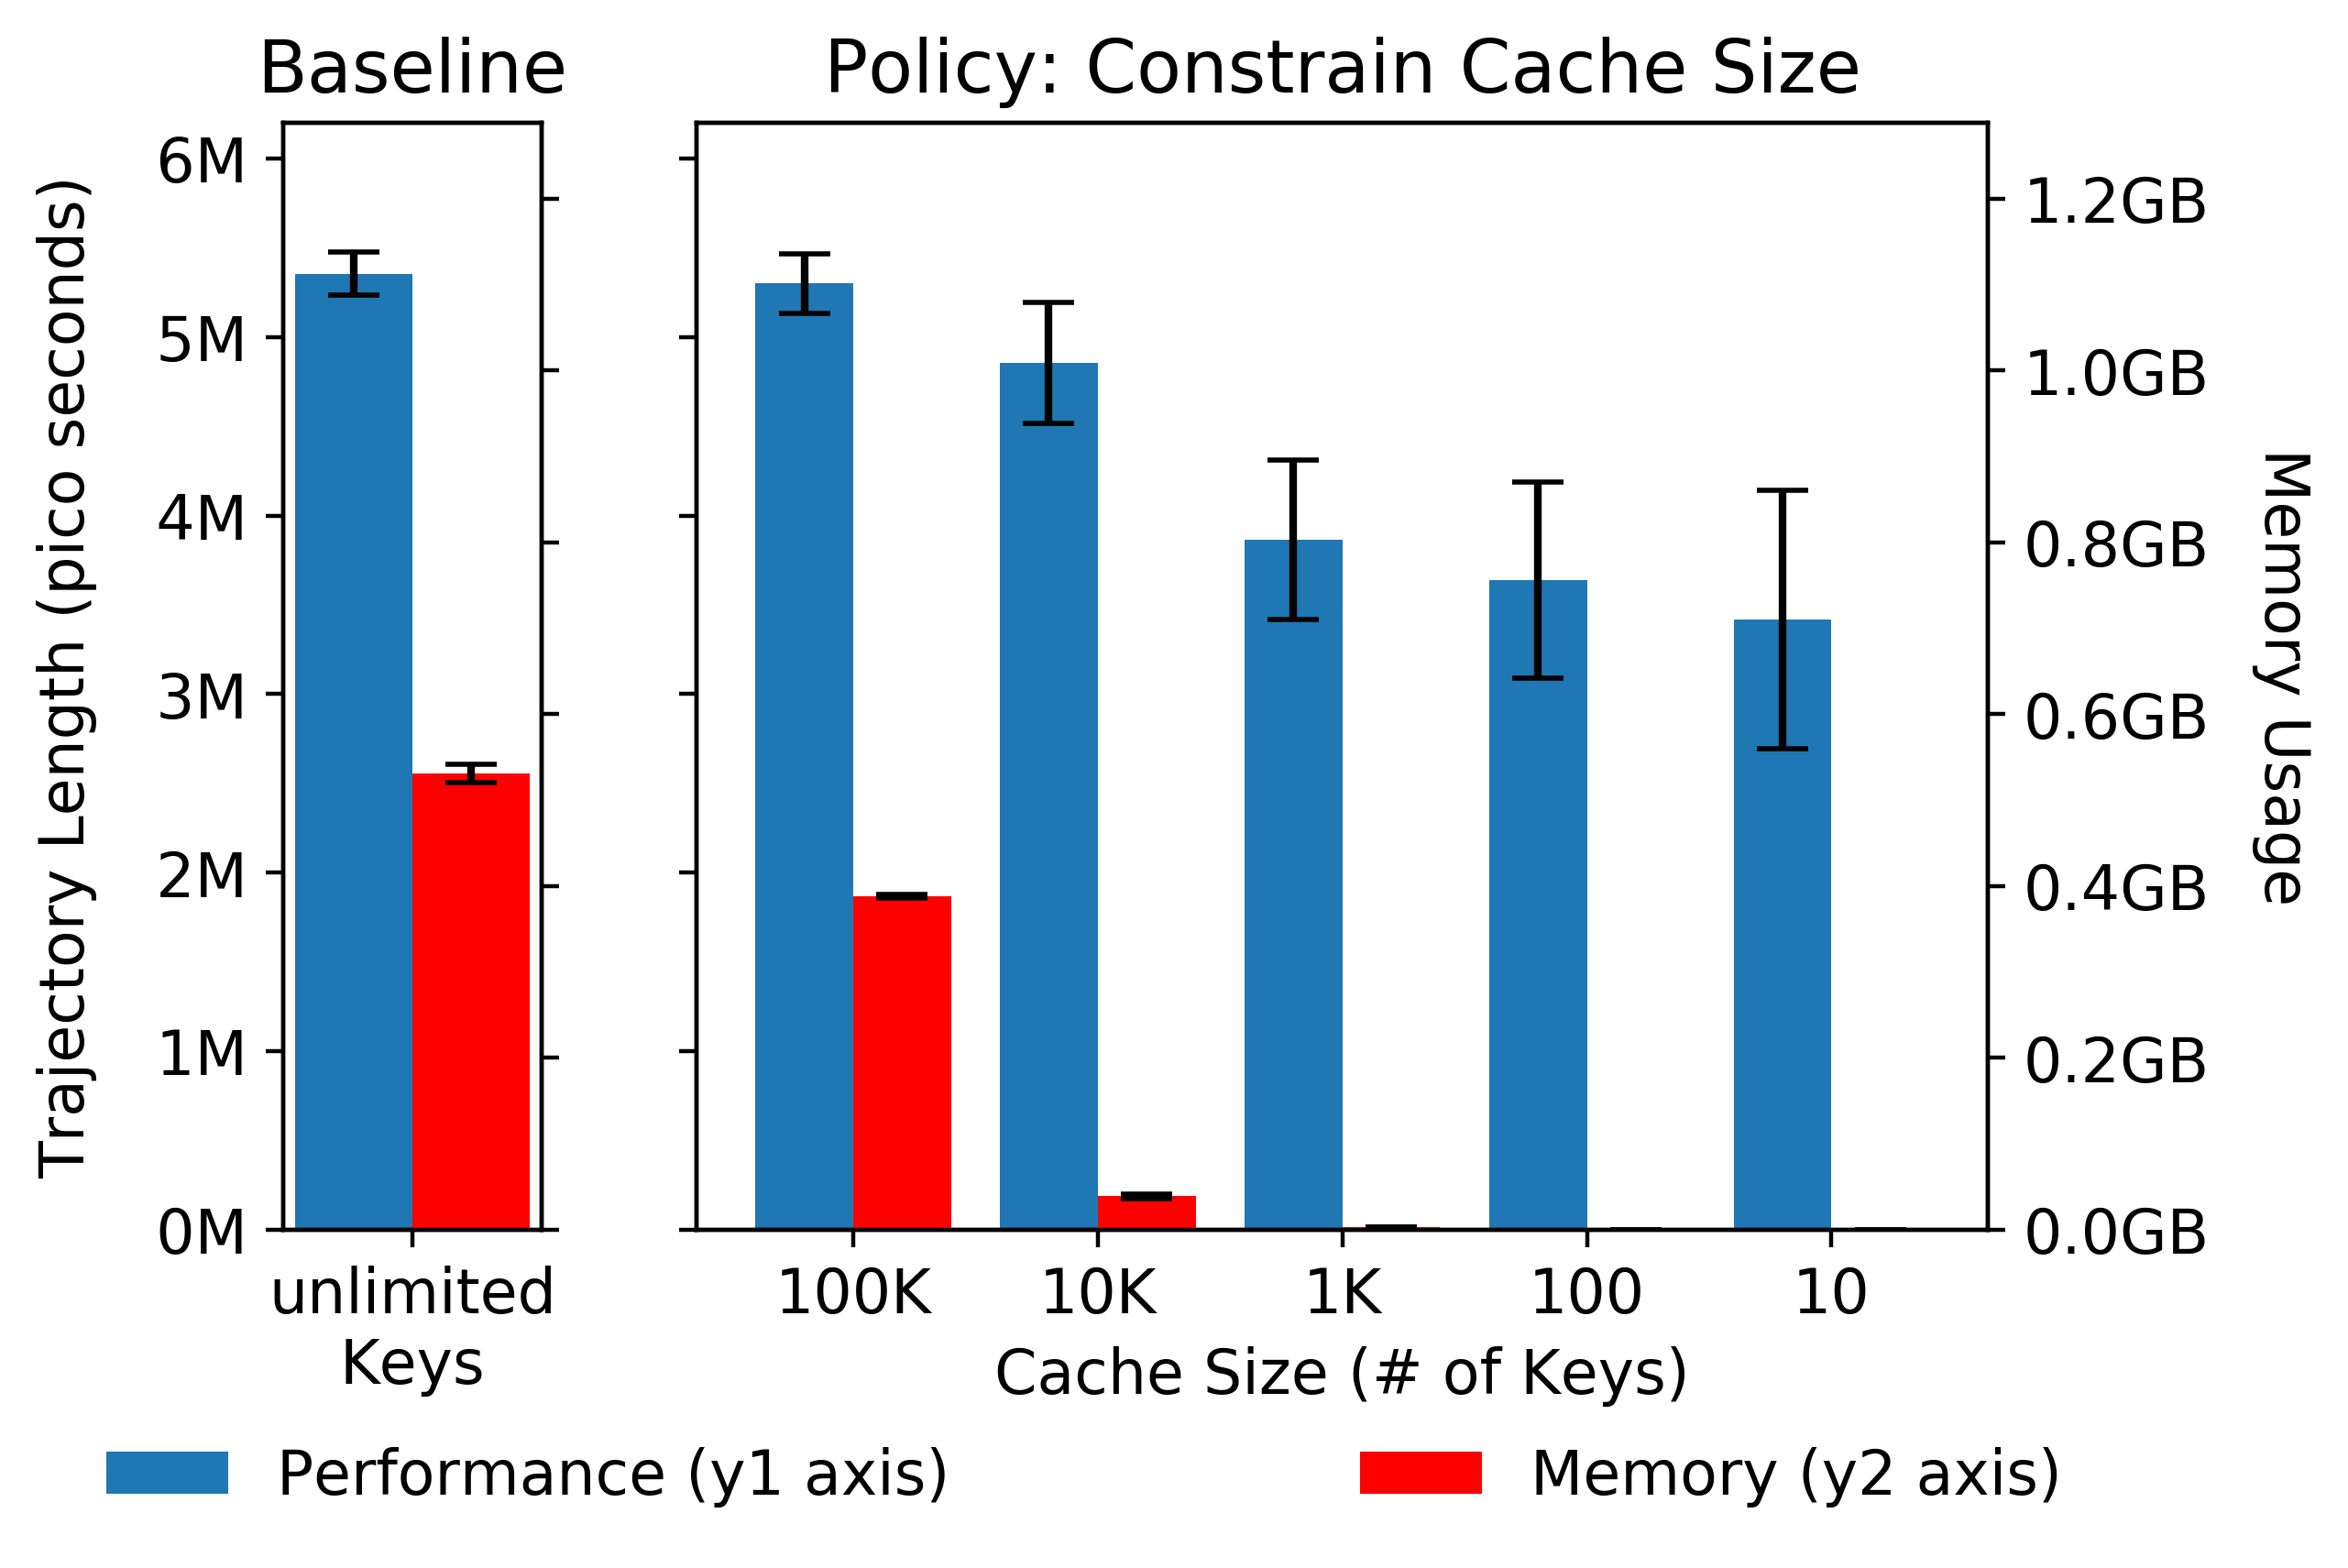
\includegraphics[width=0.5\textwidth]{figures/keyspace-analysis_cachesize.png}\\
  \caption{\label{fig:keyspace-analysis_cachesize}}
\end{figure}
\begin{figure}[tb]
  \noindent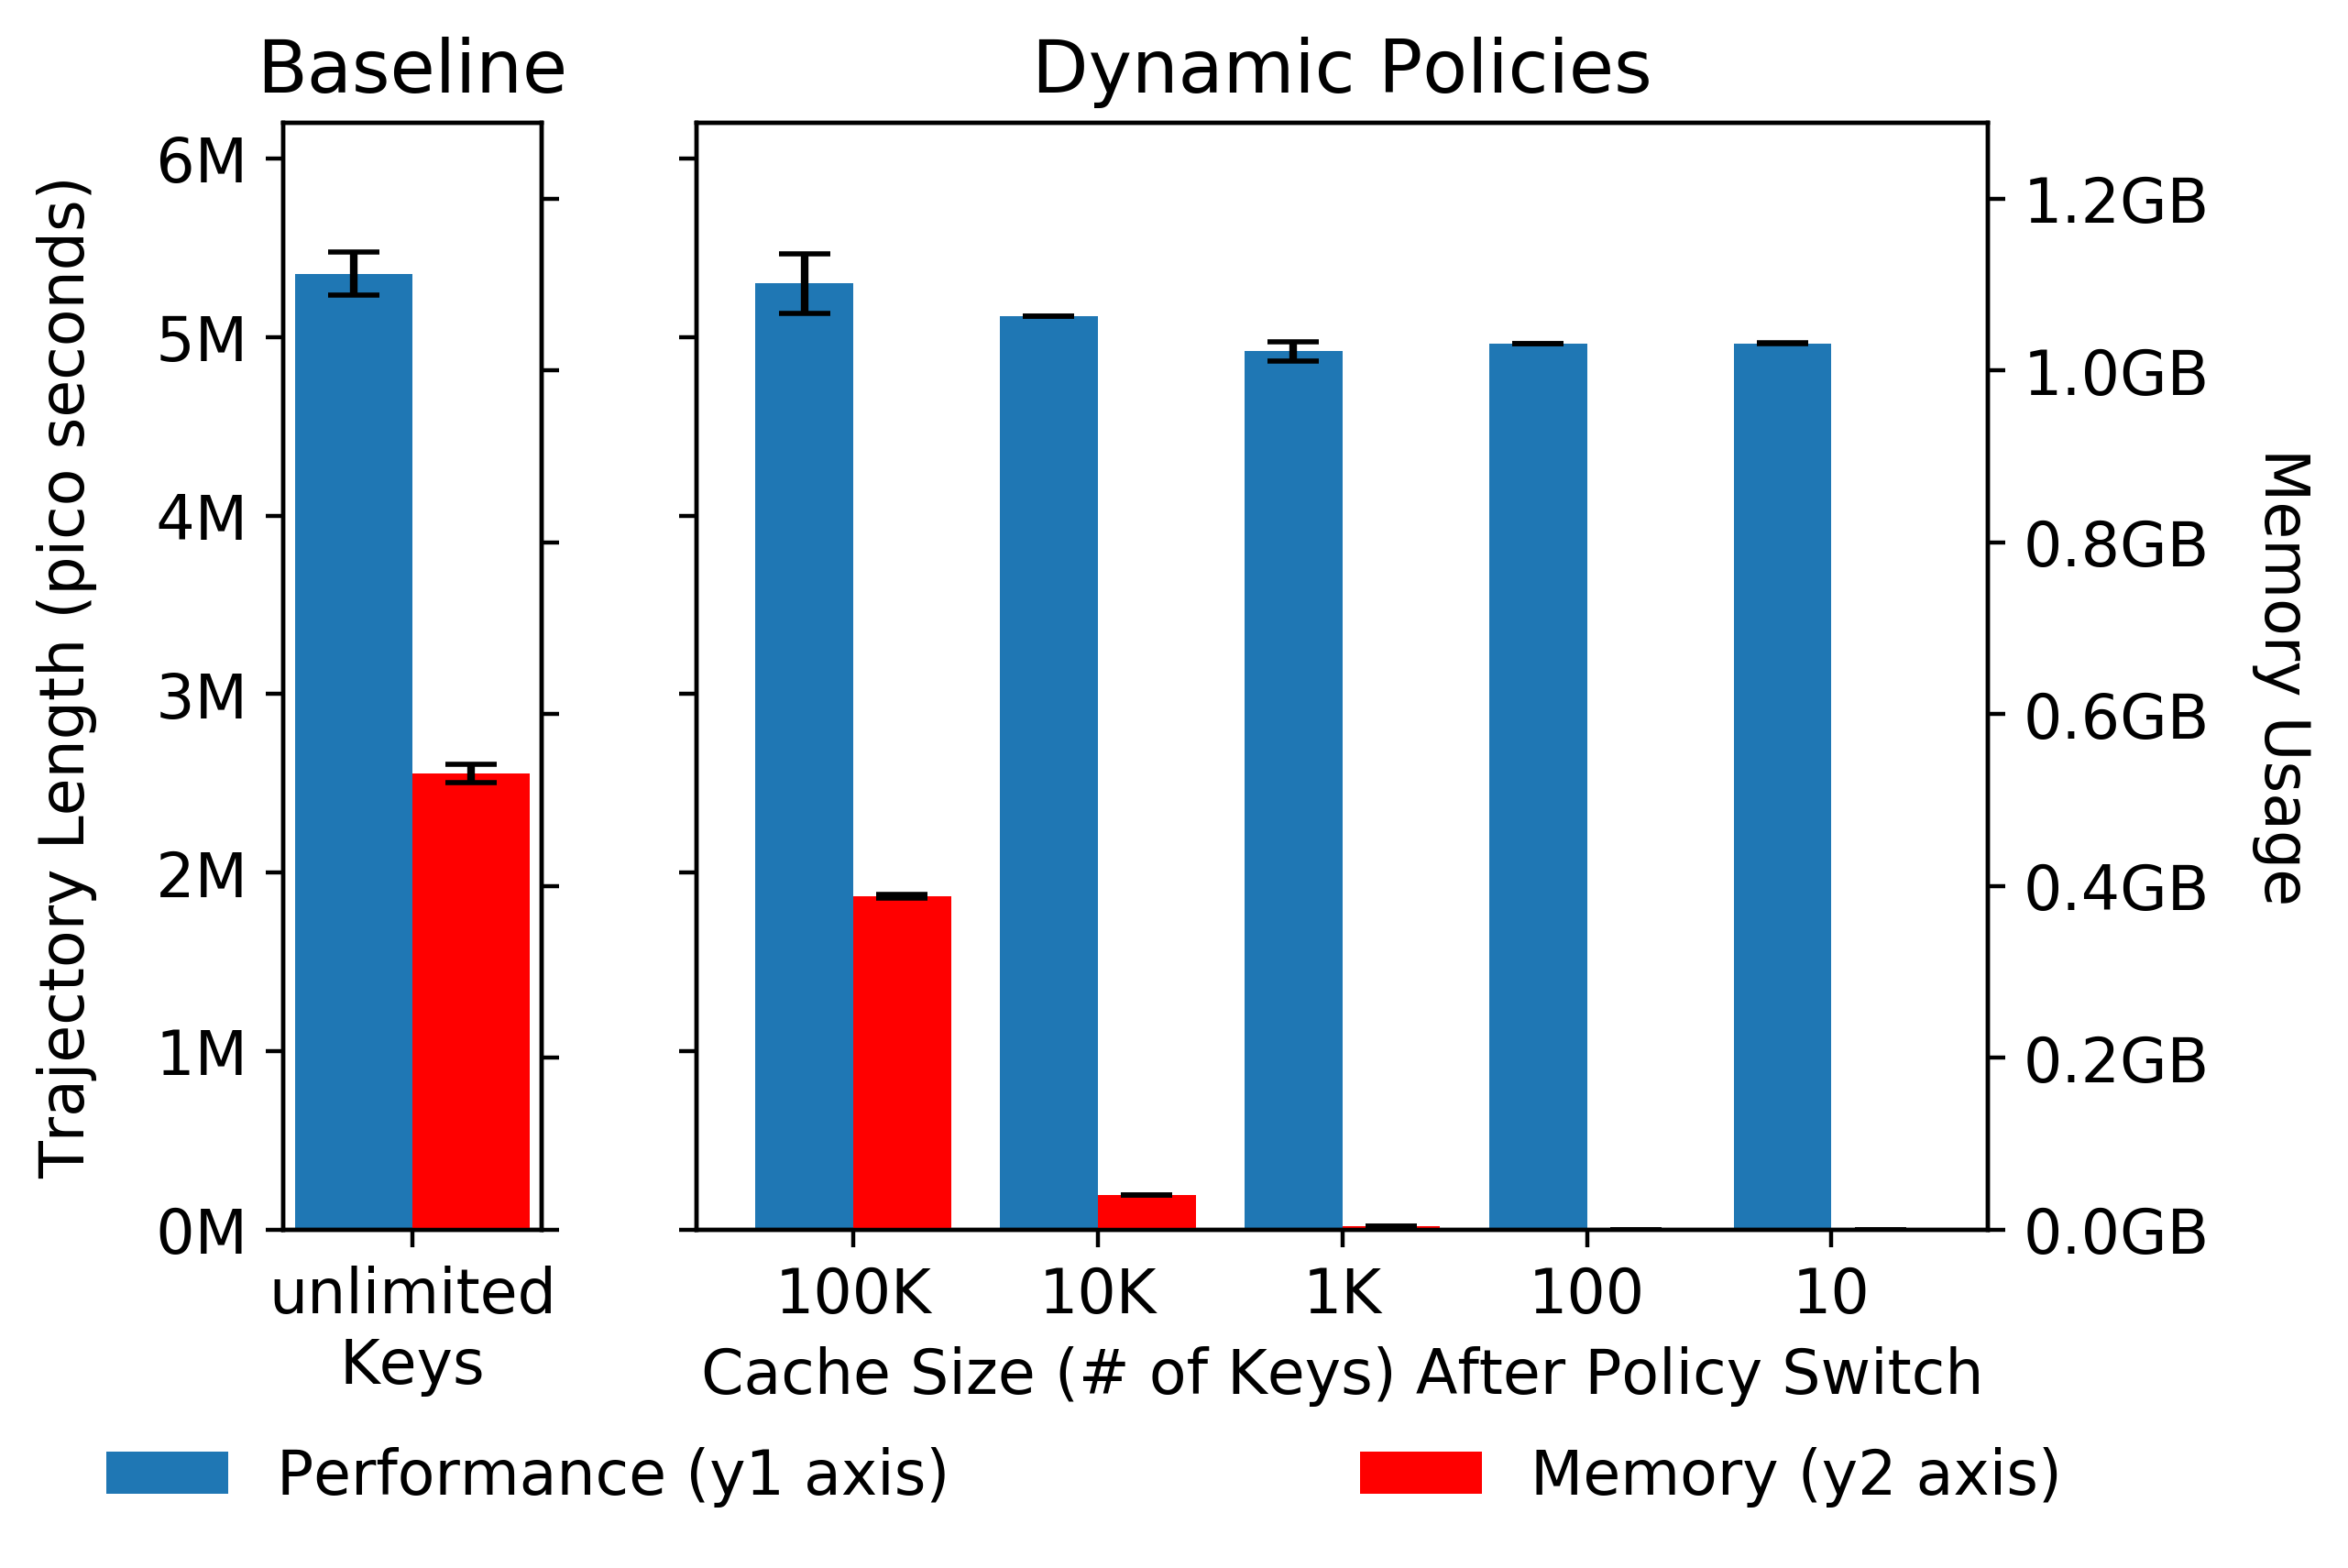
\includegraphics[width=0.5\textwidth]{figures/keyspace-analysis_cachesize-dynamic.png}\\
  \caption{\label{fig:keyspace-analysis_cachesize-dynamic}}
\end{figure}
\begin{figure}[tb]
  \noindent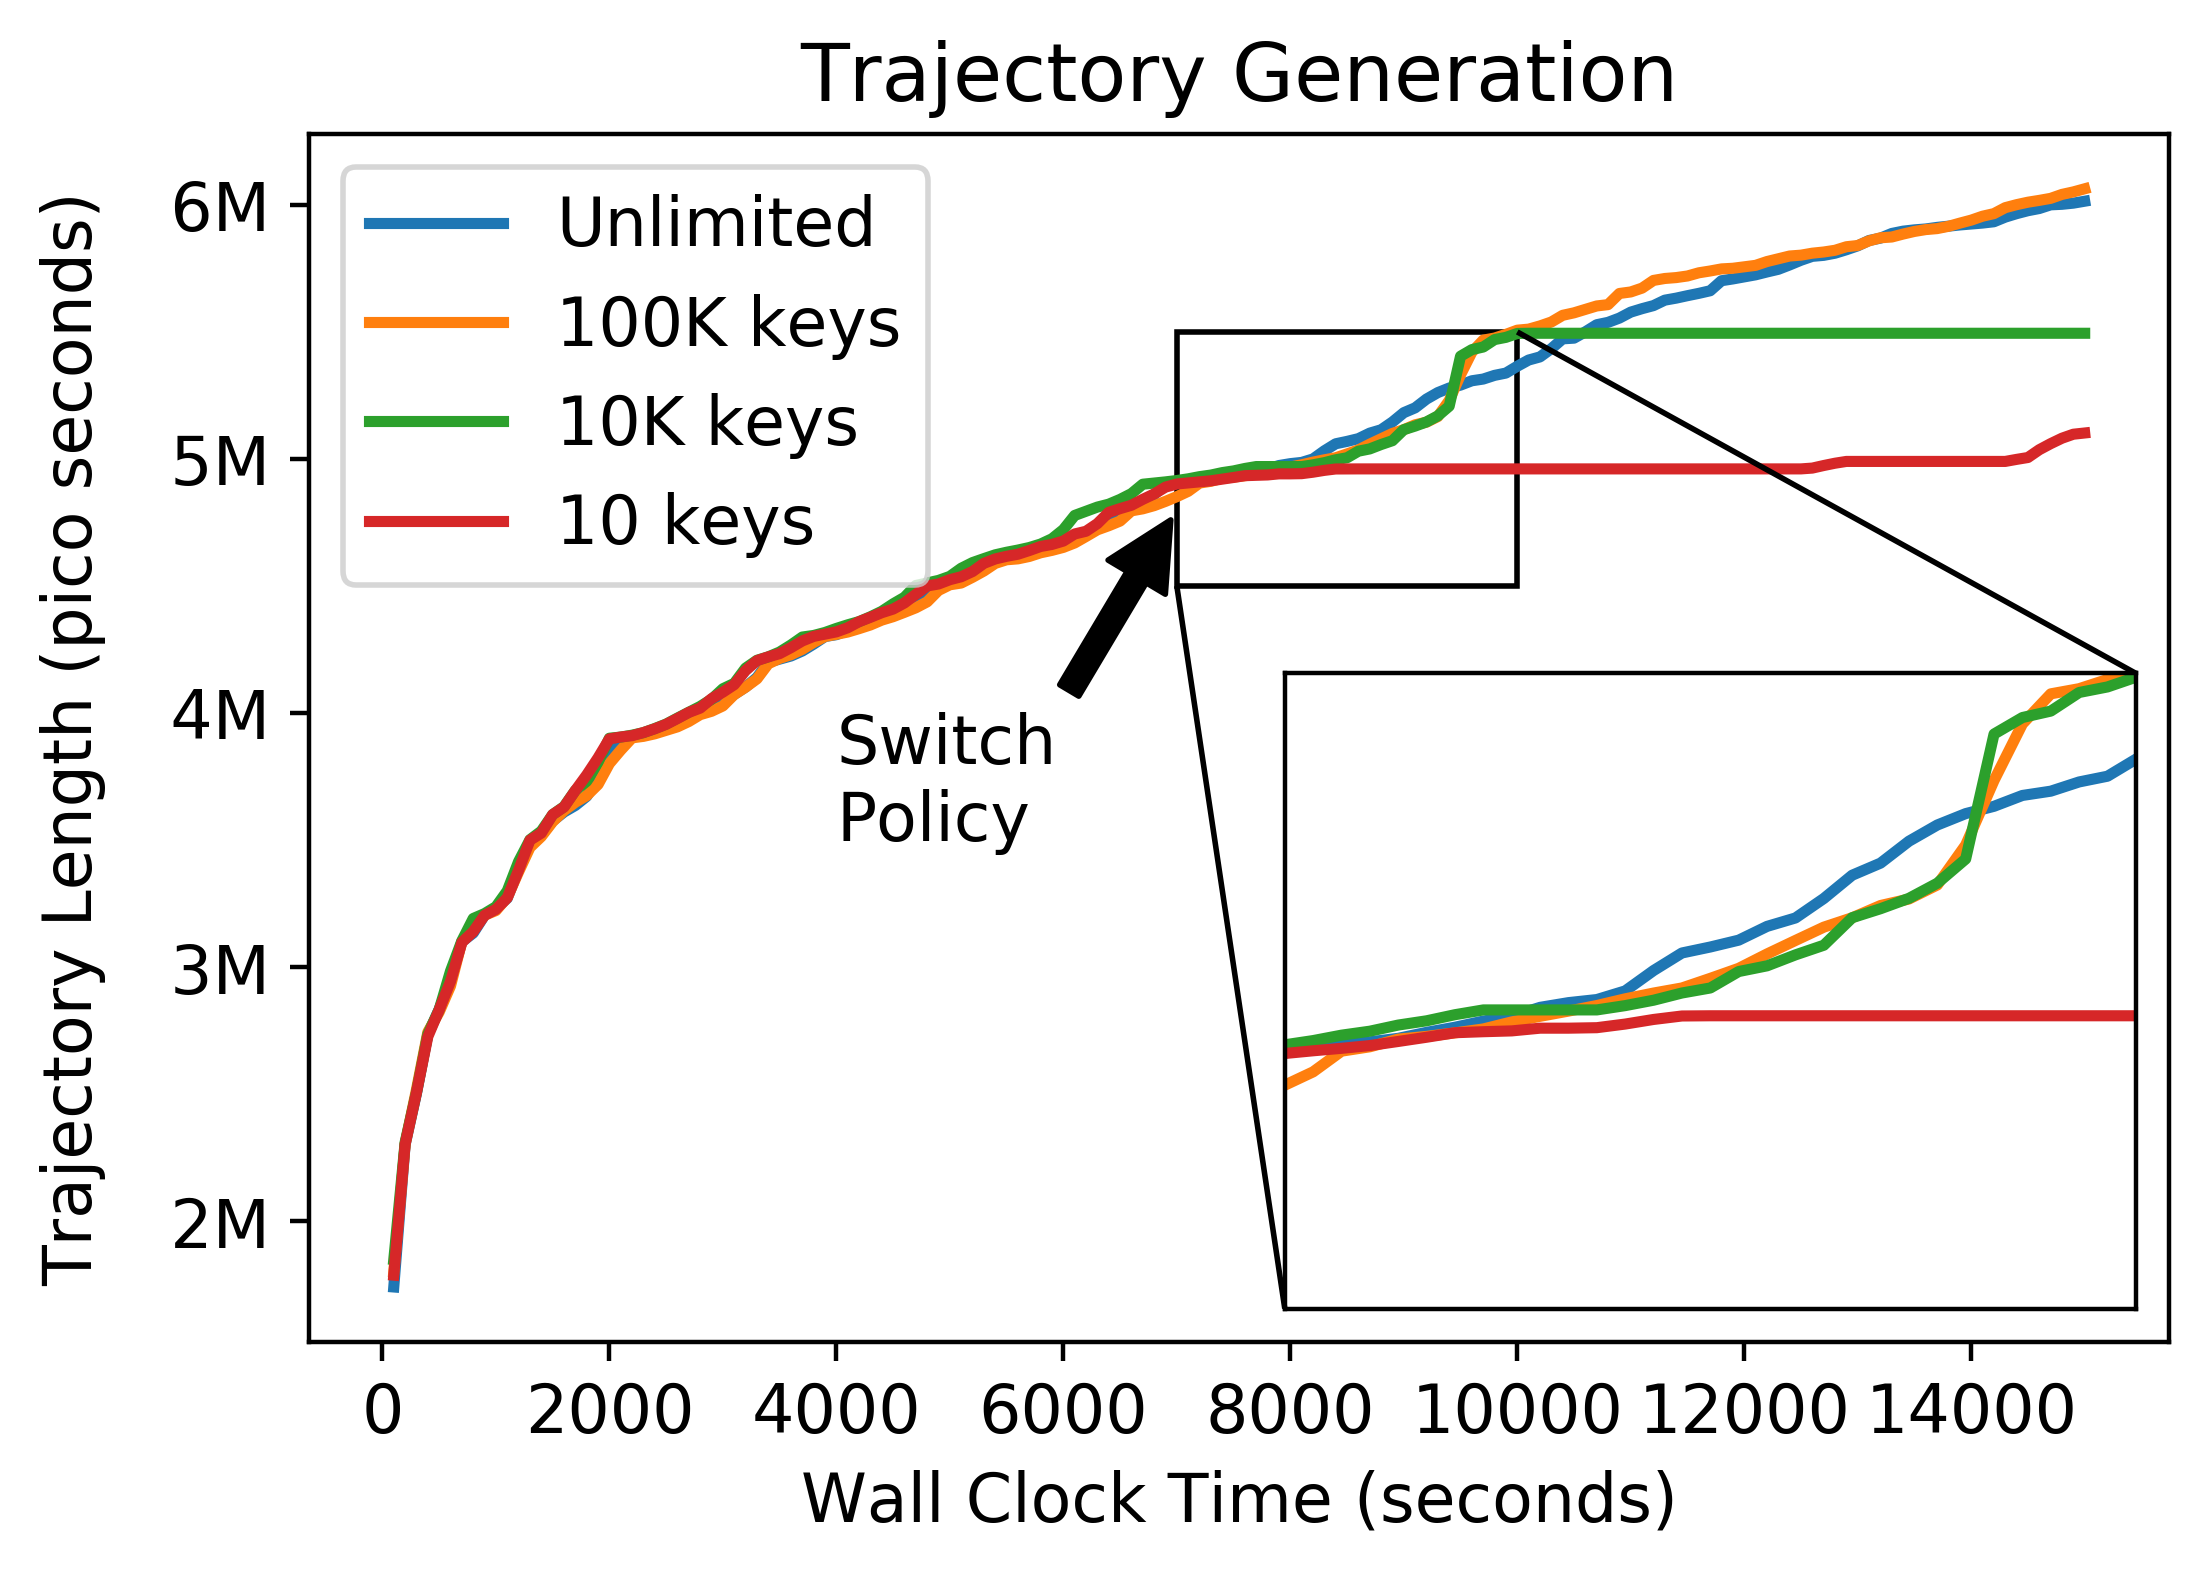
\includegraphics[width=0.5\textwidth]{figures/keyspace-analysis_cachesize-caveats.png}\\
  \caption{\label{fig:keyspace-analysis_cachesize-caveats}}
\end{figure}

